\documentclass{article}



\usepackage{arxiv}

\usepackage[utf8]{inputenc} % allow utf-8 input
\usepackage[T1]{fontenc}    % use 8-bit T1 fonts
\usepackage{hyperref}       % hyperlinks
\usepackage{url}            % simple URL typesetting
\usepackage{booktabs}       % professional-quality tables
\usepackage{amsfonts}       % blackboard math symbols
\usepackage{nicefrac}       % compact symbols for 1/2, etc.
\usepackage{microtype}      % microtypography
\usepackage{lipsum}		% Can be removed after putting your text content
\usepackage{graphicx}
\usepackage{natbib}
\usepackage{doi}



\title{Could mass eccentricity explain the formation of orbits in wind turbines?}

%\date{September 9, 1985}	% Here you can change the date presented in the paper title
%\date{} 					% Or removing it

\author{ \href{https://orcid.org/0000-0000-0000-0000}{\includegraphics[scale=0.06]{orcid.pdf}\hspace{1mm} Aljoscha Sander}\thanks{Use footnote for providing further information about author (webpage, alternative address)---\emph{not} for acknowledging funding agencies.} \\
	Energy and Sustainability Research Institute Groningen\\
	University of Groningen\\
	Groningen, the Netherlands \\
	\texttt{aljoscha.sander@rug.nl} \\
	%% examples of more authors
	\And
	\href{https://orcid.org/0000-0000-0000-0000}{\includegraphics[scale=0.06]{orcid.pdf}\hspace{1mm} Andreas Haselsteiner} \\
	\texttt{a.haselsteiner@uni-bremen.de} \\
	\And
	Bas Holman \\
	\texttt{b.holman@outlook.com}\\
	%% Address \\
	%% \texttt{email} \\
	%% \And
	%% Coauthor \\
	%% Affiliation \\
	%% Address \\
	%% \texttt{email} \\
	%% \And
	%% Coauthor \\
	%% Affiliation \\
	%% Address \\
	%% \texttt{email} \\
}

% Uncomment to remove the date
%\date{}

% Uncomment to override  the `A preprint' in the header
%\renewcommand{\headeright}{Technical Report}
%\renewcommand{\undertitle}{Technical Report}
\renewcommand{\shorttitle}{Mass eccentricity in offshore}

%%% Add PDF metadata to help others organize their library
%%% Once the PDF is generated, you can check the metadata with
%%% $ pdfinfo template.pdf
\hypersetup{
pdftitle={Could mass eccentricity explain the formation of orbits in wind turbines?},
pdfsubject={},
pdfauthor={Aljoscha Sander, Andreas Haselsteiner, Bas Holman},
pdfkeywords={First keyword, Second keyword, More},
}

\begin{document}
\maketitle

\begin{abstract}
	blablabla
\end{abstract}


% keywords can be removed
\keywords{First keyword \and Second keyword \and More}


\section{Introduction}
\label{sec:introduction}

\begin{itemize}
    \item Orbits in offshore wind turbines
    \item Different potential causes
    \item Why of relevance? Offshore wind farm installation
    \item Operations and maintenance in general
    \item -> mass eccentricity!
\end{itemize}

\clearpage

\section{System description (ALL)}
\label{sec:system}

\begin{itemize}
    \item illustration of eccentric mass due to nacelle in the hammerhead configuration + top view
    \item description of the phenomenon in words
    \item maybe another illustration with different states of the system within one cycle?
\end{itemize}

\begin{figure}[ht!]
    \centering
    \includegraphics[width=\linewidth]{manuscript/figures/loading_2.png}
    \caption{A vibration model with three degrees of freedom (DOF).}
    \label{fig:loading}
\end{figure}

\clearpage

\section{Experiment (SAN)}
\label{sec:experiment}

\subsection{Experimental Setup}

\begin{itemize}
    \item Description of the system: geometry, material properties, excitation, measurement devices
    \item different beam lengths
    \item observations (jupyter notebook)
\end{itemize}

\begin{figure}[ht!]
    \centering
    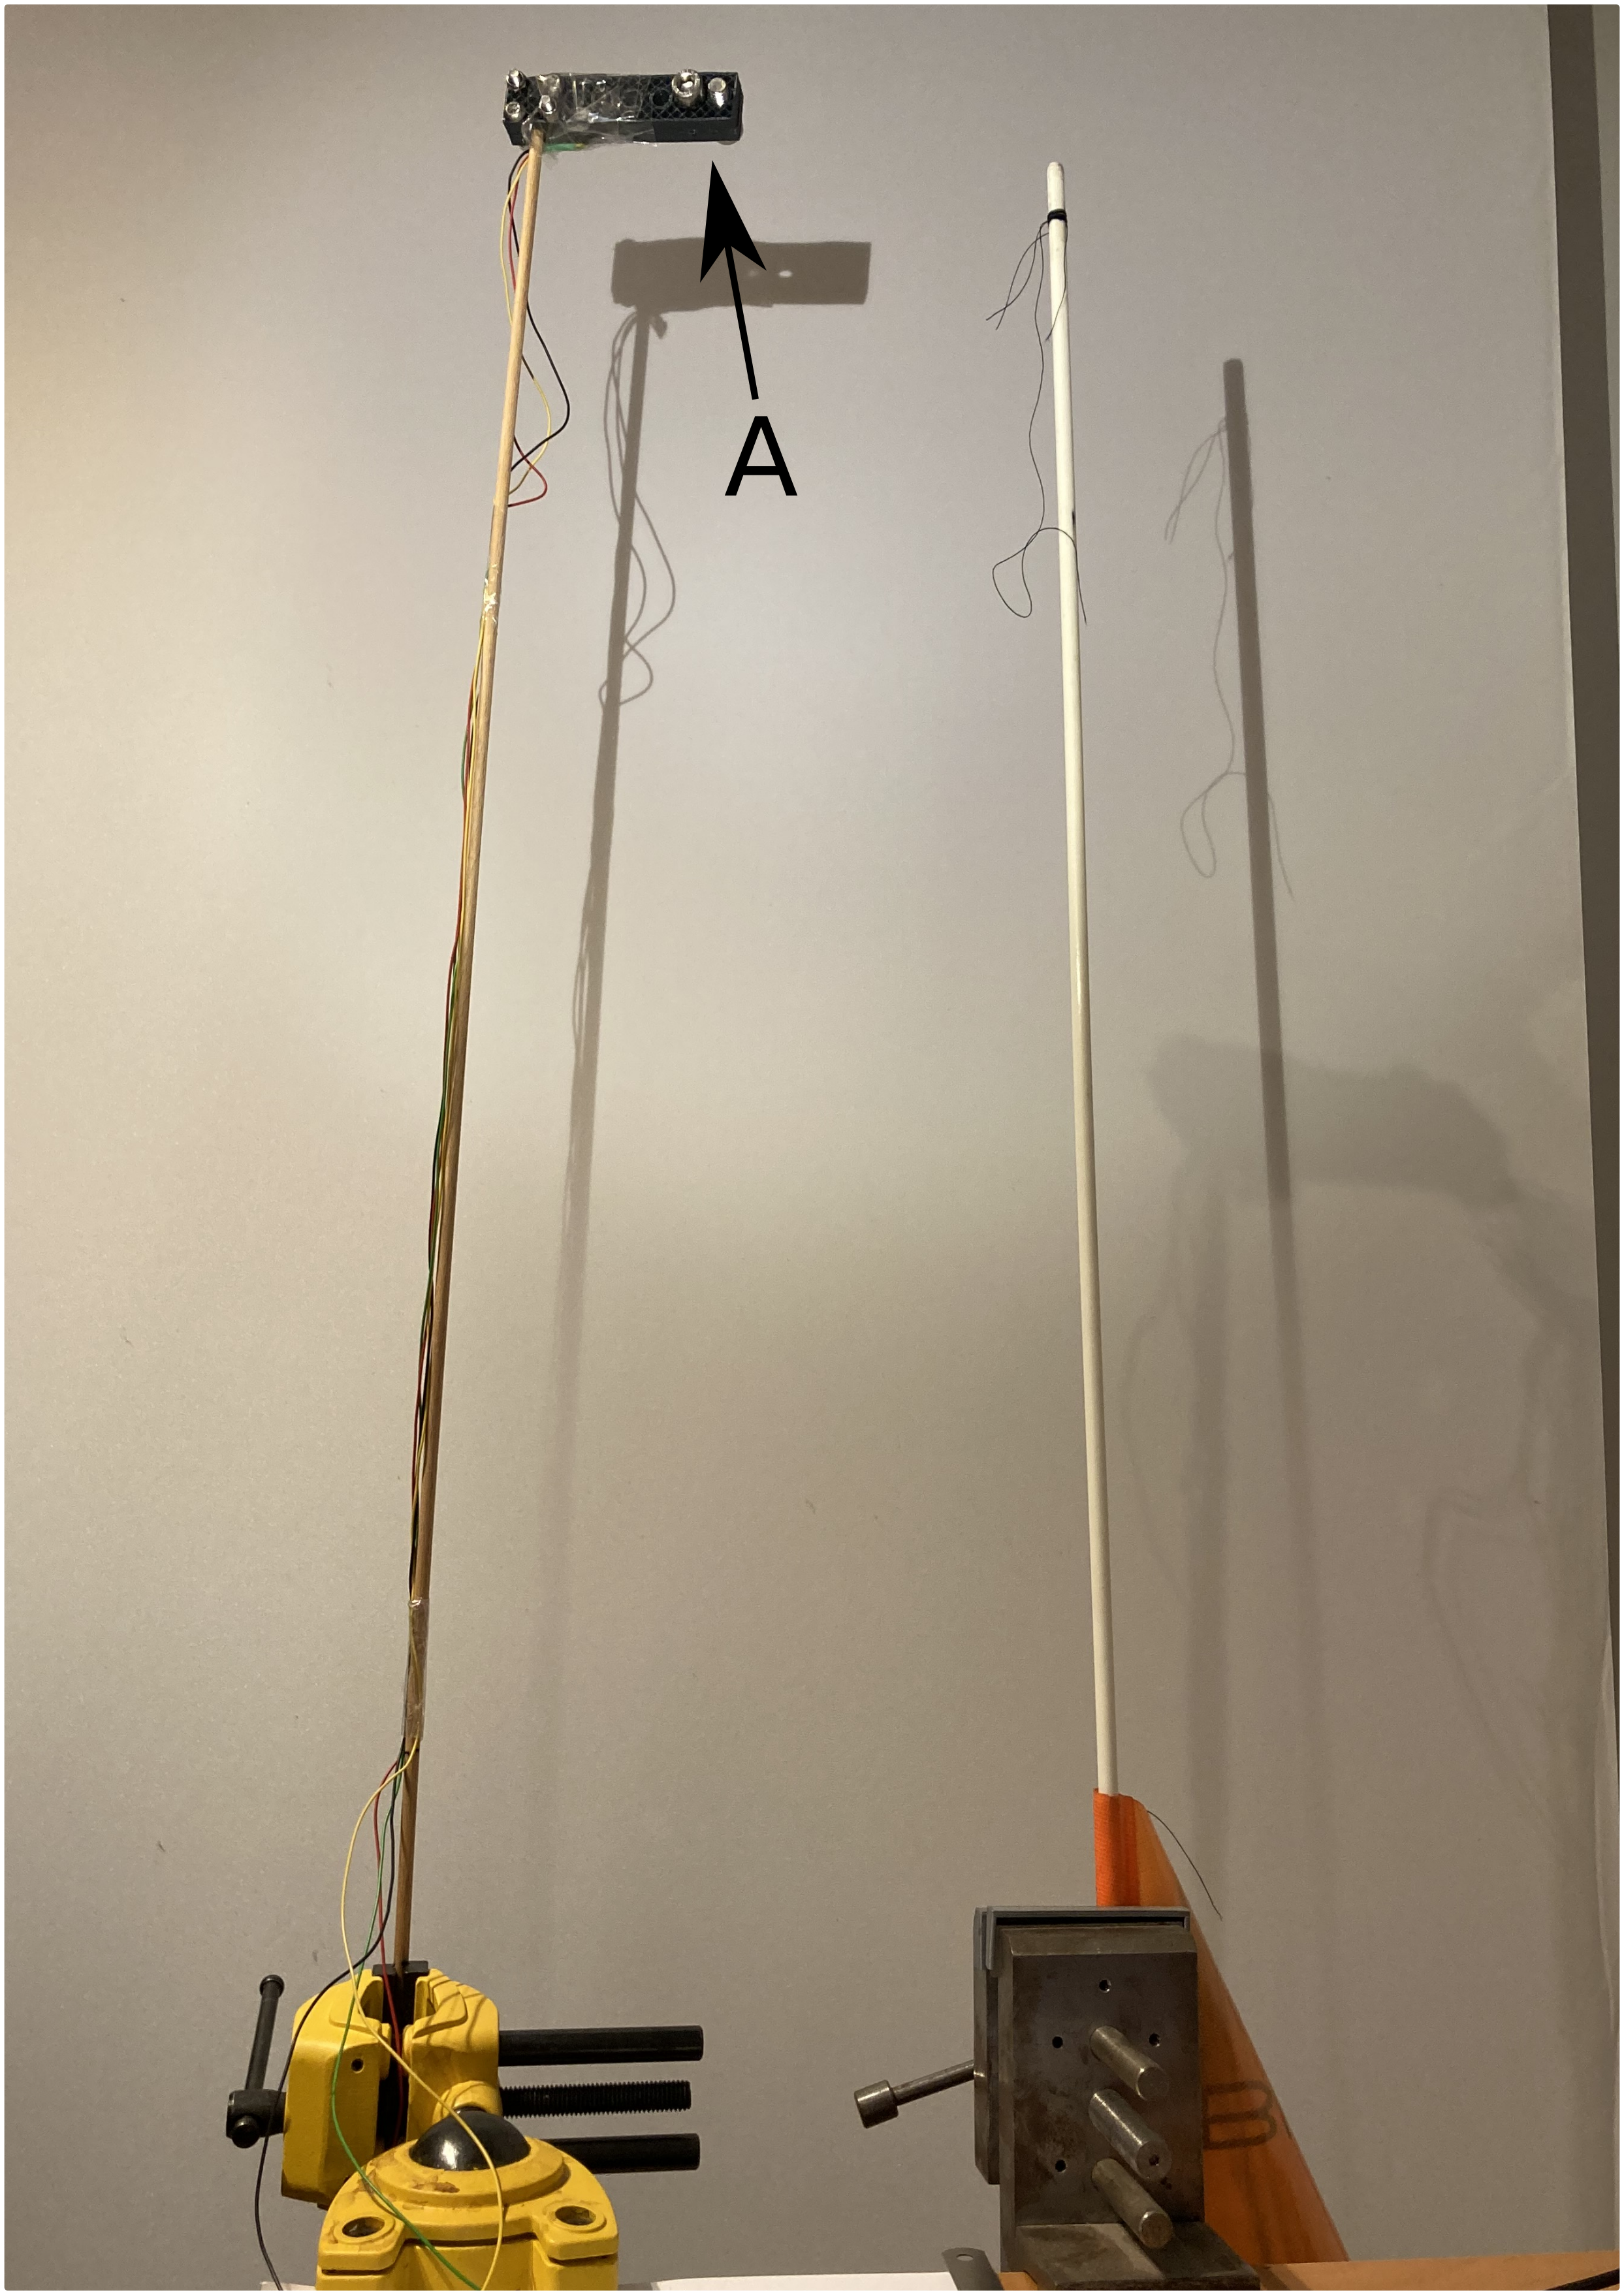
\includegraphics[width=0.5\linewidth]{manuscript/figures/setup.png}
    \caption{Experimental setup}
    \label{fig:setup}
\end{figure}

\subsection{Results}

\begin{figure}
    \centering
    \includegraphics[width=\linewidth]{results/experiment/lissajous.png}
    \caption{Lissajous figures (orbits) for three different eccentric masses}
    \label{fig:lissajous}
\end{figure}

\begin{figure}
    \centering
    \includegraphics[width=\linewidth]{results/experiment/spectrum.png}
    \caption{Caption}
    \label{fig:spectrum}
\end{figure}

\clearpage

\section{Simulations (BAS)}
\label{sec:simulations}

\subsection{Simulation Setup}

\paragraph{Model}

\paragraph{Loads}

\subsection{Simulation Results}

\paragraph{Simulations with Gravity}

\paragraph{Simulations without Gravity}

\clearpage

\section{A vibration model with three degrees of freedom}
\label{sec:3dof}

A common approach to study vibrations is to reduce the real system into a simplified model that consists of discrete components. In this approach one aims to describe the real system as simple as possible to generate the main dynamics of the real system. Many vibration phenomena can be sufficiently described with systems with only one or two degrees of freedom. Here, we present a model with three degrees of freedom that seems to capture the main dynamics of the real system.
\par 
We model the real system in two dimensions (\autoref{fig:3dof-system}). The tower's bending is modeled as a linear spring, which is connected to a fixed point, which represents the tower's foundation, and to a first body, which represents the tower's top section. The tower's torsion is modeled with a torsional spring that connects a second body with a fixed angle in the inertial reference frame. This second body is pinned to the first body such that it translates with the first body, but rotates freely. Consequently, the system's three degrees of freedom are: the first body's position in $x$ and $y$ direction and the second body's orientation.
\par 
By applying the physical laws of conservation of linear and angular momentum, we derived the equations of motions for the system (a derivation is available as supplemental material). The system's equations of motion read:
\begin{equation}
    (m_1 + m_2) \ddot{x} - \cos(\theta) m_2 d \ddot{\theta} + \sin(\theta) m_2 d \dot{\theta}^2 + k_1 x = 0,\label{eq:eom-x}
\end{equation}
\begin{equation}
    (m_1 + m_2) \ddot{y} - \sin(\theta) m_2 d \ddot{\theta} - \cos(\theta) m_2 d \dot{\theta}^2 + k_1 y = 0,\label{eq:eom-y}
\end{equation}
\begin{equation}
    (I_{zz} + m_2 d^2)\ddot{\theta} - \cos(\theta) m_2 d \ddot{x} - \sin(\theta)m_2 d \ddot{y} + k_2 \theta = 0.\label{eq:eom-theta}
\end{equation}

The equations can be arranged to have only acceleration on the left hand side:
\begin{equation}
    \ddot{x} = \frac{1}{m_1 + m_2} \left( \cos(\theta) m_2 d \ddot{\theta} - \sin(\theta) m_2 d \dot{\theta}^2 - k_1 x \right),\label{eq:eom2-x}
\end{equation}
\begin{equation}
   \ddot{y} = \frac{1}{m_1 + m_2} \left(\sin(\theta) m_2 d \ddot{\theta} + \cos(\theta) m_2 d \dot{\theta}^2 - k_1 y \right),\label{eq:eom2-y}
\end{equation}
\begin{equation}
    \ddot{\theta} = \frac{1}{I_{zz} + m_2 d^2} \left(\cos(\theta) m_2 d \ddot{x} + \sin(\theta)m_2 d \ddot{y} - k_2 \theta \right) \label{eq:eom2-theta}
\end{equation}

Several terms couple translation ($x$ and $y$) with rotation ($\theta$): for example, the acceleration in the $x$ direction, $\ddot{x}$ is equal to terms that contain $\ddot{\theta}$ and $\dot{\theta}$ (\autoref{eq:eom2-x}). Such coupling terms are necssary to appear in the equation as otherwise only linear motion would be possible -- in other words, the mass would move back and forth on a straight line.
\par 
The translational acceleration is affected by the second mass' centrifugal and Euler forces. Centrifugal force acts in the $-\hat{r}$ direction and reads, 
\begin{equation}
    m_2 d \dot{\theta}^2,
\end{equation}
and Euler force acts in the $\hat{\theta}$ direction and reads
\begin{equation}
    m_2 d \ddot{\theta}.
\end{equation}
The equation for $\ddot{\theta}$ (\autoref{eq:eom2-theta}) was derived by applying conservation of angular momentum around the center of mass $G$. The force that acts at the location where the second body is pinned to the first body depend on the first body's acceleration in $x$ and $y$ direction such that there are also coupling terms with $\ddot{x}$ and $\ddot{y}$ in the equation for $\ddot{\theta}$  (\autoref{eq:eom2-theta}).
\par 
As expected, the equations also show that if $d=0$ the coupling terms disappear:
\begin{equation}
    (m_1 + m_2) \ddot{x} = - k_1 x,
\end{equation}
\begin{equation}
   (m_1 + m_2) \ddot{y} = - k_1 y,
\end{equation}
\begin{equation}
    I_{zz}\ddot{\theta} = - k_2 \theta.
\end{equation}

\begin{figure}
    \centering
    \includegraphics{manuscript/figures/vibration_model.jpg}
    \caption{A vibration model with three degrees of freedom (DOF).}
    \label{fig:3dof-system}
\end{figure}

The vibration model can reproduce the type of motions that were measured in the table top experiment and in the offshore measurement campaign [??? maybe the offshore measurements not]. \autoref{tab:3dof-variable-values} lists the parameter values that were estimated from the table top experiment and the offshore measurement campaign.

\begin{table}[]
    \centering
    \begin{tabular}{l l l l}
    \toprule
         Quantity & Table top experiment & Offshore measurements & Unit \\
         \midrule
         $m_1$ & X & 320$\times$10$^3$ & kg\\ 
         $m_2$ & X & 450$\times$10$^3$ & kg\\ 
         $k_1$ & X & 3.4$\times$10$^6$ & N\,m$^{-1}$ \\ 
         $k_2$ & X & 3.6$\times$10$^9$ & Nm\,rad$^{-1}$ \\ 
         $d$ & X & 0.28 & m\\ 
         $I_{zz}$ & X & 3.6$\times$10$^7$ & kg\,m$^2$ \\ 
         \bottomrule
    \end{tabular}
    \caption{Values used in the 3-DOF vibration model that correspond to the table top experiment and the offshore measurements.}
    \label{tab:3dof-variable-values}
\end{table}

\clearpage

\section{Conclusion (ALL)}
\label{sec:experiment}

\begin{itemize}
    \item future work
    \item implications for offshore wind
\end{itemize}

\clearpage

\bibliographystyle{unsrtnat}
\bibliography{references}  %%% Uncomment this line and comment out the ``thebibliography'' section below to use the external .bib file (using bibtex) .


%%% Uncomment this section and comment out the \bibliography{references} line above to use inline references.
% \begin{thebibliography}{1}

% 	\bibitem{kour2014real}
% 	George Kour and Raid Saabne.
% 	\newblock Real-time segmentation of on-line handwritten arabic script.
% 	\newblock In {\em Frontiers in Handwriting Recognition (ICFHR), 2014 14th
% 			International Conference on}, pages 417--422. IEEE, 2014.

% 	\bibitem{kour2014fast}
% 	George Kour and Raid Saabne.
% 	\newblock Fast classification of handwritten on-line arabic characters.
% 	\newblock In {\em Soft Computing and Pattern Recognition (SoCPaR), 2014 6th
% 			International Conference of}, pages 312--318. IEEE, 2014.

% 	\bibitem{hadash2018estimate}
% 	Guy Hadash, Einat Kermany, Boaz Carmeli, Ofer Lavi, George Kour, and Alon
% 	Jacovi.
% 	\newblock Estimate and replace: A novel approach to integrating deep neural
% 	networks with existing applications.
% 	\newblock {\em arXiv preprint arXiv:1804.09028}, 2018.

% \end{thebibliography}


\end{document}
